\documentclass[12pt,a4paper]{article}

% ─── Page Layout ───────────────────────────────────────────────────────────────
\usepackage[a4paper, margin=0.8in, headheight=14pt]{geometry}

% ─── Fonts (XeLaTeX) ───────────────────────────────────────────────────────────
\usepackage{fontspec}
\usepackage{unicode-math}
\setmainfont{TeX Gyre Pagella}
\setmonofont[Scale=0.88]{TeX Gyre Cursor}
\setmathfont{Latin Modern Math}

% ─── Packages ──────────────────────────────────────────────────────────────────
\usepackage{xcolor}
\usepackage{colortbl}
\usepackage{titlesec}
\usepackage{enumitem}
\usepackage{tabularx}
\usepackage{booktabs}
\usepackage{array}
\usepackage{amsmath}
\usepackage{tikz}
\usetikzlibrary{shapes.geometric, arrows.meta, positioning, calc, fit, decorations.pathreplacing, patterns}
\usepackage[american]{circuitikz}
\usepackage{tcolorbox}
\tcbuselibrary{skins, breakable}
\usepackage{hyperref}
\usepackage{fancyhdr}
\usepackage{graphicx}
\usepackage{microtype}
\hyphenpenalty=10000
\exhyphenpenalty=10000
\sloppy
\usepackage{caption}
\usepackage{setspace}
\usepackage{multirow}
\usepackage{tocloft}

% ─── Q&A helper ────────────────────────────────────────────────────────────────
\newcommand{\Q}[1]{\textbf{#1}\par\noindent\ignorespaces}

% ─── Colour Palette ────────────────────────────────────────────────────────────
\definecolor{myred}{RGB}{196,30,58}
\definecolor{mydark}{RGB}{30,30,50}
\definecolor{mygreen}{RGB}{14,120,80}
\definecolor{myteal}{RGB}{0,130,140}
\definecolor{myamber}{RGB}{180,100,0}
\definecolor{mypurple}{RGB}{100,30,160}
\definecolor{mygray}{RGB}{246,247,249}
\definecolor{mgframe}{RGB}{180,185,200}
\definecolor{watermark}{RGB}{145,150,170}
\definecolor{hdrred}{RGB}{250,232,235}
\definecolor{hdrgreen}{RGB}{220,244,233}
\definecolor{hdrteal}{RGB}{220,242,244}
\definecolor{hdramber}{RGB}{253,242,215}
\definecolor{hdrpurple}{RGB}{238,228,255}
\definecolor{hdrgray}{RGB}{238,240,245}
\definecolor{rowalt}{RGB}{250,251,253}

% ─── Section Formatting ────────────────────────────────────────────────────────
\titleformat{\section}{\large\bfseries\color{myred}}{\thesection.}{0.5em}{}[\vspace{1pt}{\color{myred}\rule{\linewidth}{0.8pt}}]
\titleformat{\subsection}{\normalsize\bfseries\color{myteal}}{\thesubsection}{0.5em}{}
\titlespacing*{\section}{0pt}{18pt}{7pt}
\titlespacing*{\subsection}{0pt}{11pt}{4pt}

% ─── Paragraph ─────────────────────────────────────────────────────────────────
\setlength{\parindent}{0pt}
\setlength{\parskip}{4pt}

% ─── TOC Styling ───────────────────────────────────────────────────────────────
\renewcommand{\cfttoctitlefont}{\large\bfseries\color{myred}}
\renewcommand{\cftaftertoctitle}{\par\noindent{\color{myred}\rule{\linewidth}{0.8pt}}}
\setlength{\cftbeforetoctitleskip}{0pt}
\setlength{\cftaftertoctitleskip}{6pt}
\renewcommand{\cftsecfont}{\normalsize\bfseries\color{mydark}}
\renewcommand{\cftsecpagefont}{\normalsize\bfseries\color{mydark}}
\renewcommand{\cftsecleader}{\cftdotfill{\cftdotsep}}
\setlength{\cftbeforesecskip}{7pt}
\renewcommand{\cftsubsecfont}{\small\color{mydark}}
\renewcommand{\cftsubsecpagefont}{\small\color{mydark}}
\setlength{\cftbeforesubsecskip}{3pt}
\setlength{\cftsubsecindent}{1.4em}

% ─── Table helpers ─────────────────────────────────────────────────────────────
\renewcommand{\arraystretch}{1.45}
\setlength{\tabcolsep}{6pt}
\arrayrulecolor{mydark}
\newcolumntype{B}[1]{>{\small\bfseries\raggedright\arraybackslash}m{#1}}
\newcolumntype{Y}{>{\small\raggedright\arraybackslash}X}
\renewcommand{\tabularxcolumn}[1]{m{#1}}

% ─── Header / Footer ───────────────────────────────────────────────────────────
\pagestyle{fancy}
\fancyhf{}
\fancyhead[L]{\small\color{myred}\textbf{PE-EC802B}\;\color{mydark}--- Industrial Automation and Control}
\fancyhead[R]{\small\color{myteal}\textbf{Module 2 Notes}}
\fancyfoot[C]{\small\color{mydark}\thepage}
\fancyfoot[R]{\small\color{watermark}\textit{\copyright\ Biraj}}
\renewcommand{\headrulewidth}{0.5pt}
\renewcommand{\footrulewidth}{0.3pt}

% ─── Hyperref ──────────────────────────────────────────────────────────────────
\hypersetup{colorlinks=true, linkcolor=myteal, urlcolor=myteal,
  pdfauthor={Biraj Sarkar}, pdftitle={PE-EC802B --- Module 2 Notes}}

% ─── tcolorbox styles ──────────────────────────────────────────────────────────
\tcbset{
  tikzbox/.style={colback=mygray, colframe=mgframe, boxrule=0.6pt, arc=4pt,
    left=8pt, right=8pt, top=6pt, bottom=6pt,
    colbacktitle=mgframe, coltitle=mydark, fonttitle=\small\bfseries},
  defbox/.style={colback=hdrgreen, colframe=mygreen, boxrule=0.8pt, arc=4pt,
    left=9pt, right=9pt, top=6pt, bottom=6pt,
    colbacktitle=mygreen, coltitle=white, fonttitle=\small\bfseries},
  formulabox/.style={colback=hdrteal, colframe=myteal, boxrule=0.8pt, arc=4pt,
    left=9pt, right=9pt, top=7pt, bottom=7pt,
    colbacktitle=myteal, coltitle=white, fonttitle=\small\bfseries},
  examplebox/.style={colback=hdramber, colframe=myamber, boxrule=0.8pt, arc=4pt,
    left=9pt, right=9pt, top=6pt, bottom=6pt,
    colbacktitle=myamber, coltitle=white, fonttitle=\small\bfseries},
  masonbox/.style={colback=hdrpurple, colframe=mypurple, boxrule=0.8pt, arc=4pt,
    left=9pt, right=9pt, top=6pt, bottom=6pt,
    colbacktitle=mypurple, coltitle=white, fonttitle=\small\bfseries},
  exambox/.style={colback=hdrpurple, colframe=mypurple, boxrule=1pt, arc=5pt,
    left=10pt, right=10pt, top=8pt, bottom=8pt,
    colbacktitle=mypurple, coltitle=white, fonttitle=\bfseries,
    breakable, title after break={\textbf{Frequently Asked / Viva Questions (contd.)}}}
}
\tcbset{breakable}

% ─── TikZ styles ───────────────────────────────────────────────────────────────
\tikzset{
  block/.style={rectangle, draw=myteal, fill=hdrteal,
    text width=2.4cm, align=center, minimum height=0.95cm,
    font=\small, rounded corners=3pt, line width=0.7pt},
  redblock/.style={rectangle, draw=myred, fill=hdrred,
    text width=2.4cm, align=center, minimum height=0.95cm,
    font=\small, rounded corners=3pt, line width=0.7pt},
  sumjunc/.style={circle, draw=myamber, fill=hdramber,
    minimum size=0.62cm, font=\small, line width=0.8pt},
  arrow/.style={-Stealth, thick, color=mydark},
  line/.style={thick, color=mydark}
}

% ═══════════════════════════════════════════════════════════════════════════════
\begin{document}
% ═══════════════════════════════════════════════════════════════════════════════

\begin{center}
  {\LARGE\bfseries\color{myred} PE-EC802B --- Industrial Automation and Control}\\[5pt]
  {\normalsize\color{mydark} Semester VIII \quad$\bullet$\quad 3L:0T:0P \quad$\bullet$\quad 3 Credits}\\[3pt]
  {\normalsize\color{myteal}\textbf{Module 2 Exam Notes}}\\[3pt]
  {\small\color{mydark} CGEC \;$|$\; B.Tech ECE (2023--27) \;$|$\; \textit{Biraj Sarkar}}
\end{center}
\vspace{2pt}
\noindent{\color{myred}\rule{\linewidth}{1.5pt}}
\vspace{2pt}

\hypersetup{linkcolor=mydark}
\tableofcontents
\hypersetup{linkcolor=myteal}
\newpage

% ===============================================================================
\section{Industrial Signal Conditioning}
% ===============================================================================

Physical signals from industrial sensors are usually low-voltage ($\mu$V to mV), high-impedance, and contaminated with common-mode noise. \textbf{Signal conditioning} circuits amplify, filter, and isolate these inputs before conversion.

\subsection{1. Three-Op-Amp Instrumentation Amplifier}
An instrumentation amplifier (IA) is a specialized differential amplifier characterized by extremely high input impedance, low DC offset, and outstanding \textbf{Common-Mode Rejection Ratio (CMRR)}.

\begin{tcolorbox}[tikzbox, title={Three-Op-Amp Instrumentation Amplifier Schematic}]
\centering
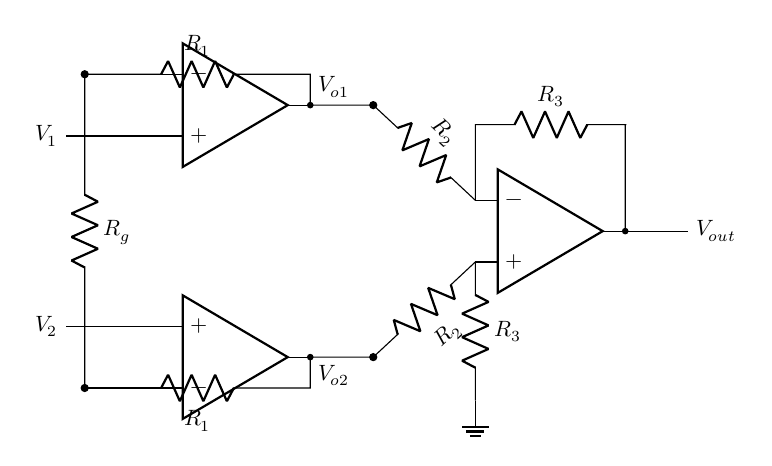
\begin{tikzpicture}[scale=0.8, transform shape]
  % Op-amps
  \draw (0, 2) node[op amp] (op1) {};
  \draw (0, -2) node[op amp, yscale=-1] (op2) {};
  \draw (5, 0) node[op amp] (op3) {};

  % Inputs
  \draw (op1.-) -- ++(-1.2, 0) coordinate (in1_minus);
  \draw (op1.+) -- ++(-1.5, 0) node[left] {$V_1$};
  \draw (op2.-) -- ++(-1.2, 0) coordinate (in2_minus);
  \draw (op2.+) -- ++(-1.5, 0) node[left] {$V_2$};

  % Resistors
  \draw (in1_minus) to[R, l=$R_1$] (op1.out |- op1.-) -- (op1.out);
  \draw (in2_minus) to[R, l_=$R_1$] (op2.out |- op2.-) -- (op2.out);
  \draw (in1_minus) to[R, l=$R_g$, *-*] (in2_minus);

  % Output of first stage nodes
  \fill (op1.out) circle (1.5pt) node[above right] {$V_{o1}$};
  \fill (op2.out) circle (1.5pt) node[below right] {$V_{o2}$};

  % Connections to second stage
  \draw (op1.out) -- ++(1.0, 0) to[R, l=$R_2$, *-] (op3.-);
  \draw (op2.out) -- ++(1.0, 0) to[R, l_=$R_2$, *-] (op3.+);

  % Feedback and reference for second stage
  \draw (op3.-) -- ++(0, 1.2) to[R, l=$R_3$] ++(2.4, 0) -| (op3.out);
  \draw (op3.+) to[R, l=$R_3$] ++(0, -2.2) node[ground] {};

  % Output
  \draw (op3.out) -- ++(1.0, 0) node[right] {$V_{out}$};
  \fill (op3.out) circle (1.5pt);
\end{tikzpicture}
\tcbset{breakable}
\end{tcolorbox}

\textbf{Mathematical Gain Derivation:}
\begin{enumerate}[label=\textbf{\arabic*.}, leftmargin=*]
  \item \textbf{First Stage (Input Buffers):} By virtual ground concept, the voltages at the inverting terminals of $A_1$ and $A_2$ are held at $V_1$ and $V_2$ respectively. Thus, the voltage drop across the gain resistor $R_g$ is:
  \[
  V_{Rg} = V_1 - V_2
  \]
  \item The current flowing through $R_g$ is $I_g = \frac{V_1 - V_2}{R_g}$. Since no current flows into the op-amp terminals, this same current $I_g$ must flow through both feedback resistors $R_1$. The voltage difference between the first-stage outputs $V_{o1}$ and $V_{o2}$ is:
  \[
  V_{o1} - V_{o2} = I_g (R_1 + R_g + R_1) = I_g (2R_1 + R_g)
  \]
  Substitute $I_g$:
  \[
  V_{o1} - V_{o2} = \left(\frac{V_1 - V_2}{R_g}\right) (2R_1 + R_g) = \left(1 + \frac{2R_1}{R_g}\right)(V_1 - V_2)
  \]
  \item \textbf{Second Stage (Differential Amplifier):} The second stage is a standard differential amplifier. Under matched resistor conditions ($R_2$ and $R_3$):
  \[
  V_{out} = \frac{R_3}{R_2}(V_{o2} - V_{o1})
  \]
  \item \textbf{Net Closed-Loop Output Voltage:} Combining the two stage equations yields:
  \begin{tcolorbox}[formulabox, title={\textbf{Instrumentation Amplifier Output Gain}}]
  \[
  V_{out} = \left(1 + \frac{2R_1}{R_g}\right)\left(\frac{R_3}{R_2}\right)(V_2 - V_1)
  \]
  \end{tcolorbox}
  By adjusting only a single external resistor $R_g$, the differential gain can be tuned across a wide range without upsetting resistor matching or input impedance.
\end{enumerate}

\subsection{2. Sallen-Key Active Filtering}
Active filters reject high-frequency noise while buffering signals. The Sallen-Key topology is the standard second-order active filter.

\textbf{Transfer Function (2nd-Order Low-Pass):}
\[
H(s) = \frac{V_{out}(s)}{V_{in}(s)} = \frac{K}{s^2(R_1 R_2 C_1 C_2) + s(R_1 C_2 + R_2 C_2 + R_1 C_1(1-K)) + 1}
\]
where $K$ is the passband gain. Sallen-Key is highly preferred due to its low component count and minimal sensitivity to op-amp bandwidth limitations.

\subsection{3. Electrical Isolation \& Protection}
Ground loops and common-mode voltage surges can damage control equipment. Isolation breaks physical copper connections while passing the signal.
\begin{itemize}[leftmargin=*, itemsep=2.5pt]
  \item \textbf{Optocouplers (Optical Isolation):} A transmitter LED converts the electrical input into light, which crosses a dielectric barrier to turn on a phototransistor on the receiver side. Provides up to $5\,$kV isolation.
  \item \textbf{Sensor Protection Circuits:} TVS (Transient Voltage Suppressor) diodes and clamping diodes shunt transient voltage spikes (such as electrostatic discharge or inductive switching surges) to power rails/ground, protecting sensitive ADC inputs.
\end{itemize}

\subsection{4. Analog-to-Digital and Digital-to-Analog Converters (ADC \& DAC)}
In computer-based automation (like PLCs or DCS), analog field signals must be digitized by an \textbf{Analog-to-Digital Converter (ADC)} for processor execution, and control outputs must be converted back to analog by a \textbf{Digital-to-Analog Converter (DAC)} to drive actuators.

\textbf{1. ADC Resolution and Quantization:}
An $N$-bit ADC maps a continuous voltage range $V_{FSR}$ to $2^N$ discrete digital states.
\begin{itemize}[leftmargin=*, itemsep=2pt]
  \item \textbf{LSB Size (Resolution):} Represents the smallest voltage change that can be resolved:
  \begin{tcolorbox}[formulabox, title={\textbf{ADC LSB Resolution}}]
  \[
  LSB = \frac{V_{FSR}}{2^N}
  \]
  \end{tcolorbox}
  \item \textbf{Quantization Error:} The error introduced by rounding a continuous voltage to the nearest discrete level. For an ideal ADC, the quantization error $e_q$ is bounded by:
  \[
  e_q \le \pm \frac{1}{2} LSB = \pm \frac{V_{FSR}}{2^{N+1}}
  \]
\end{itemize}

\textbf{2. Industrial ADC Architectures:}
\begin{itemize}[leftmargin=*, itemsep=2.5pt]
  \item \textbf{Successive Approximation Register (SAR) ADC:}
    \begin{itemize}[leftmargin=*, itemsep=1.5pt]
      \item \textit{Working:} Uses a binary search algorithm and an internal DAC to compare the input voltage against successive fractions of the reference voltage. It takes $N$ clock cycles for $N$-bit conversion.
      \item \textit{Characteristics:} Moderate speed (kSPS to MSPS), good resolution (8--18 bits), zero latency. Standard in PLC analog input modules.
    \end{itemize}
  \item \textbf{Sigma-Delta ($\Sigma\Delta$) ADC:}
    \begin{itemize}[leftmargin=*, itemsep=1.5pt]
      \item \textit{Working:} Employs oversampling, 1-bit delta-modulation, noise shaping (pushing quantization noise to high frequencies), and digital decimation filtering to retrieve ultra-precise digital representations.
      \item \textit{Characteristics:} Extremely high resolution (16--24 bits), high noise immunity, slow conversion speed. Ideal for precision weighing systems (load cells) and temperature transmitters (RTDs/Thermocouples).
    \end{itemize}
\end{itemize}

\textbf{3. Industrial DAC Architectures:}
\begin{itemize}[leftmargin=*, itemsep=2.5pt]
  \item \textbf{Binary-Weighted Resistor DAC:} Uses resistors scaled in binary powers ($R, 2R, 4R, \dots, 2^N R$). The sum of currents at the summing junction is proportional to the binary input.
    \begin{itemize}[leftmargin=*, itemsep=1.5pt]
      \item \textit{Limitation:} For high resolutions, the required ratio of resistor values becomes extremely large (e.g., $1:1024$ for 10-bit), making it practically impossible to fabricate on silicon with matched temperature coefficients.
    \end{itemize}
  \item \textbf{R-2R Ladder DAC:} Uses only two values of precision resistors ($R$ and $2R$).
    \begin{itemize}[leftmargin=*, itemsep=1.5pt]
      \item \textit{Advantage:} Highly scalable, easy to match and fabricate on silicon. It is the dominant architecture used in industrial control DAC modules.
    \end{itemize}
\end{itemize}

\textbf{4. DAC Parameters:}
\begin{itemize}[leftmargin=*, itemsep=2.5pt]
  \item \textbf{Differential Non-Linearity (DNL):} The difference between the actual step size and the ideal 1 LSB step size. A DNL $< -1\,$LSB can cause \textbf{non-monotonicity} (meaning the analog output decreases when the digital input increases).
  \item \textbf{Integral Non-Linearity (INL):} The maximum deviation of the actual transfer function from a straight line connecting the end points. Represents the overall linearity limit.
  \item \textbf{Settling Time:} The time required for the DAC output to settle within $\pm 0.5\,$LSB of its final value following a full-scale digital input transition. Limits output update rate.
\end{itemize}

% ===============================================================================
\section{Industrial Data Transmission and Noise Suppression}
% ===============================================================================

\subsection{1. 4--20 mA Current Loops}
In industrial plants, transmitting analog signals over long distances as voltages causes errors due to the resistance of the lead wires ($I R$ drop) and noise pickup. The \textbf{4--20 mA current loop} standard represents variables as current levels, making the loop immune to line resistance.

\begin{tcolorbox}[tikzbox, title={4--20 mA Industrial Current Loop Model}]
\centering
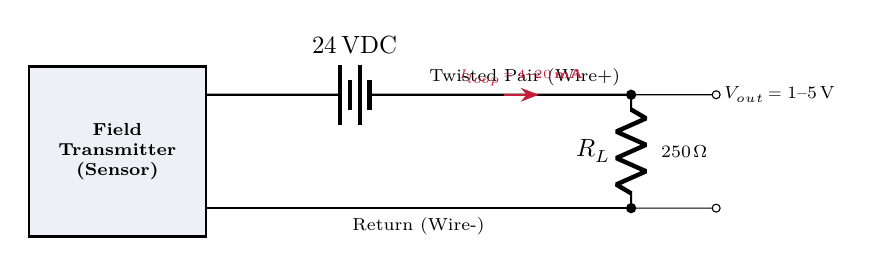
\begin{tikzpicture}[scale=0.9, transform shape]
  % Transmitter Block
  \draw[thick, fill=hdrgray] (-3.5, 1.2) rectangle (-1.0, -1.2);
  \node[font=\scriptsize\bfseries, align=center] at (-2.25, 0) {Field\\Transmitter\\(Sensor)};

  % Cable loop with loop power supply in series
  \draw[thick] (-1.0, 0.8) -- (0.4, 0.8) to[battery, l=$24\,$VDC] (1.8, 0.8) -- (5.0, 0.8);
  \node[above, font=\scriptsize] at (3.5, 0.8) {Twisted Pair (Wire+)};
  \draw[thick] (-1.0, -0.8) -- (5.0, -0.8) node[midway, below, font=\scriptsize] {Return (Wire-)};
  
  % Receiver Resistor
  \draw[thick] (5.0, 0.8) to[R, l_=$R_L$, *-*] (5.0, -0.8);
  \node[right, font=\scriptsize] at (5.3, 0) {$250\,\Omega$};
  \draw (5.0, 0.8) to[short, -o] (6.2, 0.8) node[right, font=\scriptsize] {$V_{out} = 1\text{--}5\,$V};
  \draw (5.0, -0.8) to[short, -o] (6.2, -0.8);
  
  % Loop current arrow
  \draw[-Stealth, thick, color=myred] (3.2, 0.8) -- (3.7, 0.8) node[above, midway, font=\tiny\bfseries] {$I_{loop} = 4\text{--}20\,$mA};
\end{tikzpicture}
\end{tcolorbox}

\textbf{Key Characteristics:}
\begin{enumerate}[label=\textbf{\alph*.}, leftmargin=*]
  \item \textbf{Zero Reference (4 mA):} A loop current of $4\,$mA represents the minimum scale (0\%). This "live zero" allows the controller to distinguish a true zero reading from a broken wire or loop power failure (0 mA).
  \item \textbf{Full Scale (20 mA):} Represents the maximum scale (100%).
  \item \textbf{Receiver Conversion:} At the controller side, the loop current passes through a precision $250\,\Omega$ load resistor $R_L$ to convert the current back into a voltage for the ADC:
  \[
  V_{out} = I_{loop} \times R_L
  \]
  \begin{itemize}[leftmargin=*, itemsep=2pt]
    \item For $I_{loop} = 4\,\text{mA} \Rightarrow V_{out} = 4\,\text{mA} \times 250\,\Omega = 1\,\text{V}$.
    \item For $I_{loop} = 20\,\text{mA} \Rightarrow V_{out} = 20\,\text{mA} \times 250\,\Omega = 5\,\text{V}$.
  \end{itemize}
  The resulting voltage range is a standard $1\text{--}5\,$V.
\end{enumerate}

\subsection{2. RS-485 Differential Data Transmission}
For digital communication in noisy industrial environments (e.g., Modbus protocol), RS-485 is the standard.
\begin{itemize}[leftmargin=*, itemsep=2.5pt]
  \item \textbf{Differential Signaling:} Routes data on two complementary lines ($A$ and $B$). The receiver detects only the difference $V_A - V_B$. Common-mode noise coupled onto the cable affects both lines equally and is rejected.
  \item \textbf{Termination Resistors:} A $120\,\Omega$ resistor is placed at both physical ends of the twisted pair network to match the cable's characteristic impedance, preventing signal reflections that corrupt data.
\end{itemize}

\subsection{3. Grounding and Shielding}
\begin{itemize}[leftmargin=*, itemsep=2.5pt]
  \item \textbf{Ground Loops:} When multiple devices are grounded at different physical locations, differences in ground potential drive a stray current through the ground loop wire, creating noise. Mitigated by using a single-point star ground or isolating signal paths.
  \item \textbf{Electrostatic Shielding:} Enclosing signal conductors in a conductive copper braid or foil shield connected to ground to shunt capacitive noise currents. The shield must be grounded at \textbf{one end only} to avoid creating a ground loop.
\end{itemize}

% ===============================================================================
\section{Errors, Calibration, and Uncertainty}
% ===============================================================================

\subsection{1. Error Categorization}
\begin{itemize}[leftmargin=*, itemsep=2.5pt]
  \item \textbf{Systematic (Deterministic) Errors:} Consistently bias measurements in one direction (e.g., calibration drift, scale offset, loading errors). Can be compensated for via calibration.
  \item \textbf{Random (Stochastic) Errors:} Caused by unpredictable, statistical fluctuations (e.g., thermal noise, electromagnetic interference). Analyzed using probability and mitigated by averaging.
\end{itemize}

\subsection{2. Calibration (Zero and Span Adjustments)}
Calibration is the process of adjusting a sensor's output to match known reference inputs.
\begin{itemize}[leftmargin=*, itemsep=2.5pt]
  \item \textbf{Zero Adjustment:} Shifts the entire calibration curve vertically to set the output to the correct zero value (e.g., setting output to 4 mA when input pressure is 0 psi).
  \item \textbf{Span (Gain) Adjustment:} Tilts the calibration curve by adjusting its slope to set the correct full-scale value (e.g., setting output to 20 mA when input pressure is at maximum).
\end{itemize}

\subsection{3. Uncertainty Propagation}
When a quantity $Y$ is calculated from independent measured values $X_1, X_2, \dots, X_N$ using a function $Y = f(X_1, X_2, \dots, X_N)$, the absolute uncertainty $u_Y$ is:
\begin{tcolorbox}[formulabox, title={\textbf{Uncertainty Propagation Equation}}]
\[
u_Y = \sqrt{\sum_{i=1}^N \left(\frac{\partial f}{\partial X_i} u_{X_i}\right)^2}
\]
\end{tcolorbox}
where $u_{X_i}$ is the standard uncertainty of variable $X_i$.

\newpage

% ===============================================================================
% QUICK REVISION PAGE
% ===============================================================================
\begin{center}
  {\large\bfseries\color{myred} Quick Revision --- Module 2}\\[3pt]
  {\small\color{mydark} Signal Conditioning $|$ PE-EC802B}
\end{center}
\noindent{\color{myred}\rule{\linewidth}{1.2pt}}
\vspace{4pt}

\begin{tcolorbox}[formulabox, title={\textbf{Key Formulas at a Glance}}]
\renewcommand{\arraystretch}{1.35}
\begin{tabularx}{\linewidth}{B{5.2cm} X}
Instrumentation Amp Gain & $V_{out} = \left(1 + \frac{2R_1}{R_g}\right)\left(\frac{R_3}{R_2}\right)(V_2 - V_1)$ \\[4pt]
Sallen-Key LPF Cut-off Freq & $f_c = \frac{1}{2\pi \sqrt{R_1 R_2 C_1 C_2}}$ \\[4pt]
4--20 mA Loop Volt Conversion & $V_{out} = I_{loop} \times R_L \quad (\text{For PT100/Transmitters})$ \\[4pt]
Uncertainty Propagation & $u_Y = \sqrt{\sum \left(\frac{\partial f}{\partial X_i} u_{X_i}\right)^2}$ \\[4pt]
RS-485 Term. Resistance & $R_T = Z_0 \approx 120\,\Omega$ \\[4pt]
ADC LSB Resolution & $LSB = V_{FSR} / 2^N$ \\[4pt]
ADC Quantization Error & $e_q \le \pm \frac{1}{2} LSB = \pm \frac{V_{FSR}}{2^{N+1}}$ \\
\end{tabularx}
\end{tcolorbox}

\begin{tcolorbox}[defbox, title={\textbf{One-Line Definitions}}]
\begin{itemize}[leftmargin=*, itemsep=2pt, topsep=0pt]
  \item \textbf{Instrumentation Amplifier:} A high-gain differential amplifier with extremely high input impedance and CMRR.
  \item \textbf{Live Zero:} Representing the minimum measurement value by a non-zero current (4 mA) to detect wire breaks.
  \item \textbf{Ground Loop:} An undesirable current loop formed when two points in a circuit are grounded at different potentials.
  \item \textbf{Optocoupler:} A device that uses a light path to transmit signals across an electrical isolation barrier.
  \item \textbf{Span Adjustment:} Calibration step that alters the gain (slope) of the measurement system.
  \item \textbf{Zero Adjustment:} Calibration step that adds a constant bias (offset) to shift the calibration curve.
  \item \textbf{Quantization Error:} The round-off error introduced when a continuous analog voltage is mapped to a discrete digital code.
  \item \textbf{Monotonicity:} A DAC property where the analog output always increases (or remains constant) as the digital input code increases.
\end{itemize}
\end{tcolorbox}

\begin{tcolorbox}[tikzbox, title={\textbf{Industrial Transmission \& Grounding Comparisons}}]
\centering
\par\noindent
\renewcommand{\arraystretch}{1.3}
\begin{tabularx}{\linewidth}{|B{3.0cm}|Y|Y|}
\hline
\textbf{Property} & \textbf{4--20 mA Current Loop} & \textbf{0--10 V Voltage Signaling} \\ \hline
\textbf{Noise Immunity} & Extremely High (immune to line $IR$ drop) & Low (susceptible to electromagnetic noise) \\ \hline
\textbf{Distance Limit} & Up to $3\,$km (limited by loop supply voltage) & Short distances ($<10\,$m, due to line drops) \\ \hline
\textbf{Line Break Detect} & Yes (current falls to 0 mA) & No (cannot distinguish open wire from 0 V) \\ \hline
\textbf{Wiring Cost} & Low (simple twisted pair) & High (requires shielded cables) \\ \hline
\end{tabularx}

\vspace{0.3cm}
\begin{tabularx}{\linewidth}{|B{3.0cm}|Y|Y|}
\hline
\textbf{Property} & \textbf{Single-Point Grounding} & \textbf{Multi-Point Grounding} \\ \hline
\textbf{Configuration} & All grounds connect to a single star point & Devices ground locally to the nearest chassis/earth \\ \hline
\textbf{Ground Loop Risk} & None (no duplicate return paths) & High (ground potential differences drive loops) \\ \hline
\textbf{Best Frequency} & Low frequency ($< 1\,$MHz) & High frequency ($> 10\,$MHz) \\ \hline
\end{tabularx}
\end{tcolorbox}

\begin{tcolorbox}[exambox, title={\textbf{Frequently Asked / Viva Questions}}]
\begin{enumerate}[leftmargin=*, itemsep=4pt]
  \item \Q{Why does the first stage of an instrumentation amplifier have a common-mode gain of unity?}
    In the first stage, the two buffers $A_1$ and $A_2$ are connected via $R_g$. If a common-mode voltage $V_{cm}$ is applied to both inputs ($V_1 = V_2 = V_{cm}$), the voltage across $R_g$ is zero. Hence, no current flows through $R_g$ or $R_1$. The output voltages are $V_{o1} = V_{o2} = V_{cm}$. The differential output is zero, and the common-mode gain is exactly 1.
  \item \Q{Why is 4-20 mA current loop transmission preferred over voltage transmission?}
    Current loop signals are immune to voltage drops caused by long wire resistance ($IR$ drops) and contact resistances. Furthermore, the loop current is unaffected by electromagnetic noise induced in the cabling, making it highly robust in industrial plants.
  \item \Q{Explain the "live zero" concept in 4-20 mA current loops.}
    By setting the zero-point measurement to 4 mA (instead of 0 mA), any physical wire break or power failure causes the current to drop to 0 mA. The PLC controller detects this 0 mA state as a "Loop Fail" alarm rather than a valid zero-scale reading.
  \item \Q{What is the purpose of RS-485 termination resistors, and where are they placed?}
    Termination resistors ($120\,\Omega$) match the cable's characteristic impedance. They are placed at the two extreme physical ends of the RS-485 communication line to prevent electrical signal reflections, which cause data corruption at high speeds.
  \item \Q{Why must a cable shield be grounded at only one end?}
    If a shield is grounded at both ends, any potential difference between the two grounds will drive a current through the shield conductor. This current induces noise in the internal signal wires via magnetic coupling, defeating the purpose of the shield. Grounding it at one end prevents ground loops while maintaining electrostatic shielding.
  \item \Q{State the difference between zero error and span error.}
    A zero error is a constant offset that shifts the entire calibration curve vertically, causing the same error magnitude across the full measurement range. A span error is a gain error that alters the slope of the curve, resulting in an error that increases proportionally with the input value.
  \item \Q{Compare SAR and Sigma-Delta ADCs in terms of speed, resolution, and typical industrial application.}
    SAR (Successive Approximation Register) ADCs offer moderate-to-high speed (up to a few MSPS) and moderate-to-high resolution (8--18 bits) with zero latency, making them ideal for general PLC analog inputs. Sigma-Delta ($\Sigma\Delta$) ADCs offer extremely high resolution (16--24 bits) through oversampling and noise shaping but are much slower, making them ideal for precision sensors like load cells and temperature transmitters.
  \item \Q{Explain the difference between DNL and INL in DACs.}
    DNL (Differential Non-Linearity) measures the deviation of an individual step size from the ideal 1 LSB value; a DNL $< -1\,$LSB can cause non-monotonicity. INL (Integral Non-Linearity) measures the maximum deviation of the actual transfer function from the ideal straight line, representing the overall linearity error of the DAC.
\end{enumerate}
\end{tcolorbox}

\end{document}
